\begin{frame}{Loop Freedom}
    \begin{center}
        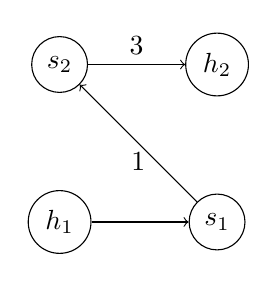
\begin{tikzpicture}[node distance={20mm},main/.style = {draw, circle}]
            \node[main] (h1)  {$h_1$};
            \node[main] (s1) [right of=h1]  {$s_1$};
            \node[main] (s2)  [above of=h1] {$s_2$};
            \node[main] (h2) [right of=s2]  {$h_2$};
            \draw[->] (h1) --  (s1);
            \draw[->] (s1) --  node[below]{1} (s2);
            \draw[->] (s2) --  node[above]{3} (h2);
        \end{tikzpicture}
        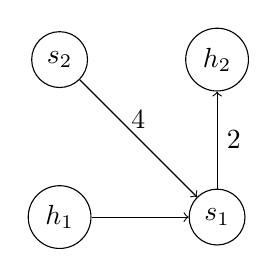
\begin{tikzpicture}[node distance={20mm},main/.style = {draw, circle}]
            \node[main] (h1)  {$h_1$};
            \node[main] (s1) [right of=h1]  {$s_1$};
            \node[main] (s2) [above of=h1] {$s_2$};
            \node[main] (h2) [right of=s2]  {$h_2$};
            \draw[->] (h1) --  (s1);
            \draw[->] (s1) -- node[right]{2} (h2);
            \draw[->] (s2) -- node[above]{4} (s1);
        \end{tikzpicture}
    \end{center}
    Property:
    \begin{itemize}
        \item Property: no forwarding loop
    \end{itemize}
    Current Behavior:
    \begin{enumerate}
        \item Replace path 3 with 4
    \end{enumerate}
\end{frame}

\begin{frame}
    \begin{center}
        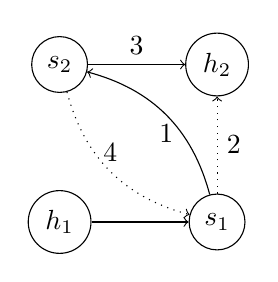
\begin{tikzpicture}[node distance={20mm},main/.style = {draw, circle}]
            \node[main] (h1)  {$h_1$};
            \node[main] (s1) [right of=h1]  {$s_1$};
            \node[main] (s2)  [above of=h1] {$s_2$};
            \node[main] (h2) [right of=s2]  {$h_2$};
            \draw[->] (h1) --  (s1);
            \draw[->] (s1) edge[bend right]  node[below]{1} (s2);
            \draw[->] (s2) --  node[above]{3} (h2);
            \draw[dotted,->] (s1) -- node[right]{2} (h2);
            \draw[dotted,->] (s2) edge[bend right]  node[above]{4} (s1);
        \end{tikzpicture}
        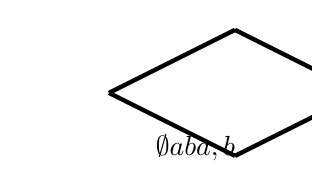
\begin{tikzpicture}[scale=0.8]
            \crd{0}{0}{$\emptyset$}
            \crd[left]{-2}{1}{$\s{a}$}
            \crd[right]{2}{1}{$\s{b}$}
            \crd[right]{0}{2}{$\s{a,b}$}
            \draw [ultra thick] (0,0) -- (2,1);
            \draw [ultra thick] (0,0) -- (-2,1);
            \draw [ultra thick] (-2,1) -- (0,2);
            \draw [ultra thick] (2,1) -- (0,2);
        \end{tikzpicture}
    \end{center}
    Events:
    \begin{itemize}
        \item $a$: Replace path 3 with 4
        \item $b$: Replace path 1 with 2
    \end{itemize}
    Counterexample: $\sigma = \s{a}$
\end{frame}
